\section{Digital-Analog-Wandler (DAC)}
\subsection{Parallelverfahren (Voltage Scalung)}
\textbf{Spannungs-DAC}: 
Serie von identischen Widerständen. Vorteil dieses DAC ist die garantierte Stetigkeit, dafür werden $2^n$ Widerstände und Schalter benötigt. Dafür wird genau ein Schalter geschlossen. Dabei wird $R1$ die Widerstände oberhalb des geschlossenr Schalter, $R2$ die unterhalb.
\begin{center}
	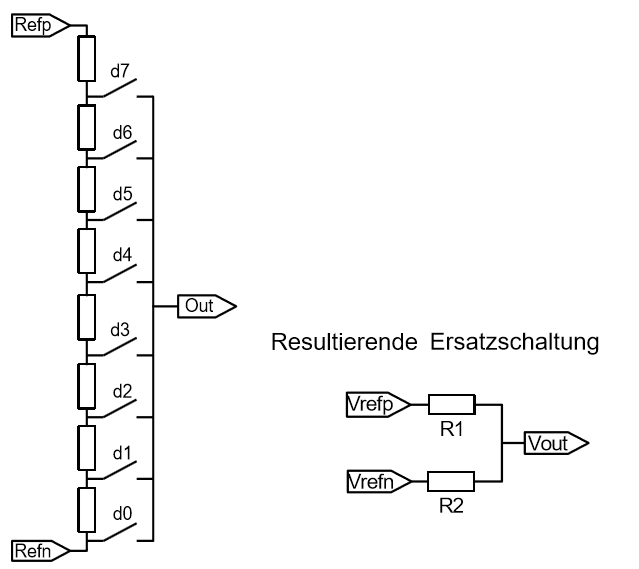
\includegraphics[width=0.7\columnwidth]{Images/dac_parallel}
\end{center}
\textbf{Beispiel:} D7 geschlossen. $V_{OUT} = (V_{refp} - V_{refn})\cdot\frac{7R}{8R}$
~\\ ~\\
\textbf{Strom-DAC}: mit Datenwort $D$
\[
I_{OUT} = D \cdot \frac{V_{REF}}{R}
\]

\subsection{Wägeverfahren}
Dieses Verfahren braucht nur $N$ Widerstände und Schalter, ist dafür nicht garantiert stetig. Am einfachsten kann dies mit den Leitwerten des Widerstands gerechnet werden $G_0 = \frac{1}{8}R$
\begin{center}
	\includegraphics[width=0.7\linewidth]{Images/wägeverfahren}
\end{center}
\begin{align*}
	V_{OUT} &= G_0\cdot \left(\frac{2^0 \cdot B_0 + 2^1 \cdot B_1 +2^2 \cdot B_2 + 2^3 \cdot B_3}{2^4}\right)\\ &\cdot (V_{refp} - V_{refn}) + V_{refn}
\end{align*}

~\\
\textbf{Charge-Scaling}
Anstatt Widerstände können auch Kapazitäten verwendet werden. Aber um eine Last zu betreiben, braucht es immer noch ein Opamp Ausgangsbuffer.\\
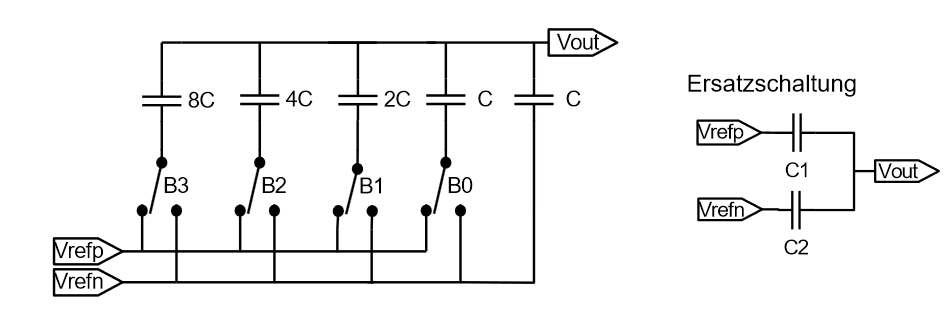
\includegraphics[width=\columnwidth]{Images/chargescaling}
\begin{align*}
	C_1 &= B_3\cdot 8C + B_2\cdot4C + B_1\cdot2C + B_0\cdot C\\	
	C_2 &= !B_3\cdot 8C + !B_2\cdot4C + !B_1\cdot2C + !B_0\cdot C\\
	V_{out} &= \frac{C_1}{C_1 + C_2}\cdot (V_{refp} - V_{refn}) +V_{refn}
\end{align*}

\textbf{R-2R}\\
Von rechts nach Links werden Widerstände zusammen addiert. Daraus erfolgt eine Gewichtung für jeden Schalter $k$. Durch die gewichteten Widerstände wird dann der Strom $2^k\cdot I_0$ erzeugt. Mit dem Opamp wird dieser Strom wieder in eine Spannung umgewandet.
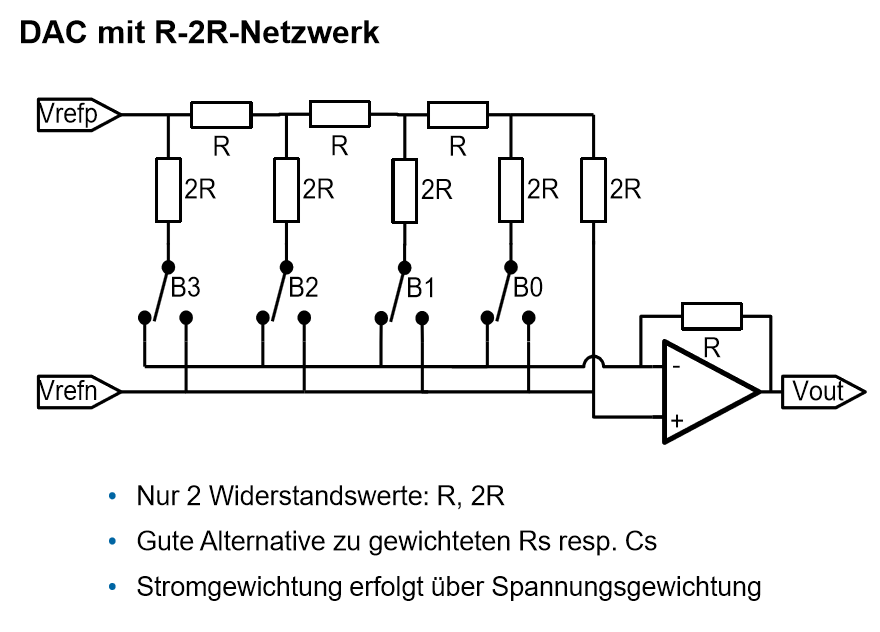
\includegraphics[width=\linewidth]{Images/r-2r}
\[
V_{out} = -(\underbrace{V_{refp} - V_{refn}}_{V_{DD}})\cdot \left(\frac{1}{1}\cdot B_0 + \frac{1}{2}\cdot B_1+ \frac{1}{4}\cdot B_2 + \cdots\right)
\]

\subsection{Zählverfahren}
Dieses Verfahren kann mit einem simplen PWM erzeugt werden, dafür benötigt man sehr viel Zeit. Die Umschaltung erfolgt über einen Digitalteil, mittels einem Tiefpass-Filter kann ein DC Spannung erzeugt werden. 
\begin{center}
	\includegraphics[width=0.6\columnwidth]{Images/zählverfahren}
\end{center}
\[
V_{OUT} = V_{REF}\cdot\underbrace{\frac{n}{N}}_\text{DutyCycle}
\]

\subsubsection{DAC Fehler}
\begin{enumerate}[nosep]
	\item Offset-Fehler
	\item Verstärkungs-Fehler
	\item Integral Nichtlinearität INL
	\item Differentielle Nichtlinearität DNL
\end{enumerate}

\subsubsection{Verzögerungszeit, Settling Time}
Zeit, bis das Ausgangssignal innerhlab des Fehlerbandes liegt sollte etwa $\pm0.5$ Quantisierungsschritte dauern.
\begin{center}
	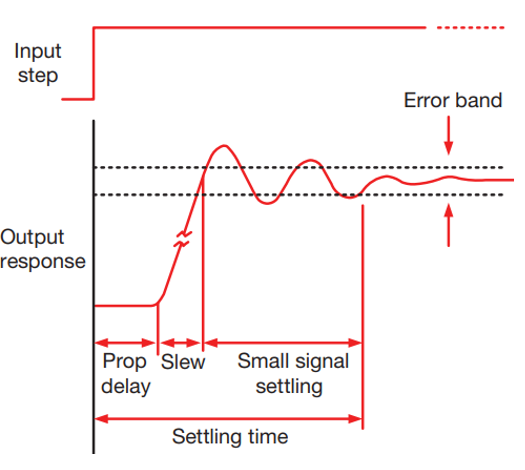
\includegraphics[width=0.5\columnwidth]{Images/settling_imte}
\end{center}


